
%%%%%%%%%%%%%%%%%%%%%%%%%%%%%%%%%%%%%%%%%%%%%%%%%%%%%%%%%%%
\section{Experiment}\label{sec:expResults}
%%%%%%%%%%%%%%%%%%%%%%%%%%%%%%%%%%%%%%%%%%%%%%%%%%%%%%%%%%%



%\subsection{Hardware System}


Our experiments are on centimeter-scale hardware systems called \emph{kilobots}.  These allows us to emulate a variety of dynamics, while enabling a high degree of control over robot function, the environment, and data collection. The kilobot, from \cite{Rubenstein2012,rubenstein2014programmable} is a low-cost robot designed for testing collective algorithms with large numbers of robots. It is available as an open source platform or commercially from~\cite{K-Team2015}.  Each robot is approximately 3 cm in diameter, 3 cm tall, and uses two vibration motors to move on a flat surface at speeds up to 1 cm/s.  Each robot has one ambient light sensor that is used to implement \emph{phototaxis},  moving towards a light source. 
In these experiments as shown in Fig.~\ref{fig:setup}, we used $n$=97 kilobots, a glass-covered 1.5 m$\times$1.2 m whiteboard as the workspace, and eight 30W LED floodlights arranged 1.5 m above the plane of the table at the $\{N,NE,E,SE,S,SW,W,NW\}$ vertices of a 6 m square centered on the workspace. The lights were controlled using an Arduino Uno board connected to an 8-relay shield.  Above  the table, an overhead machine vision system tracks the position of the swarm.


\begin{figure}
\begin{center}
	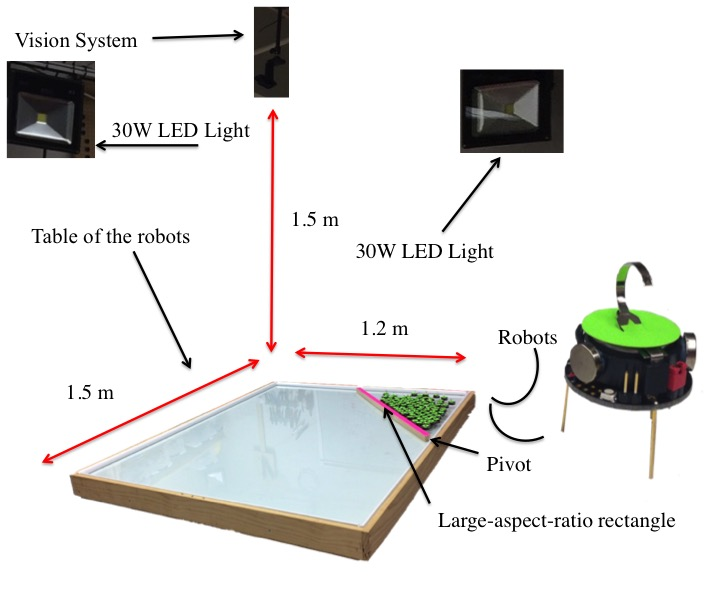
\includegraphics[width=.9\columnwidth]{SetUp.jpg}
\end{center}
\vspace{-1em}
\caption{\label{fig:setup}
Hardware platform:  table with 1.5$\times$1.2 m workspace, surrounded by eight remotely triggered 30W LED floodlights, with an overhead machine vision system.
}
\vspace{-1.5em}
\end{figure}

The experiments from Section \ref{sec:simulation}.a were repeated using this physical swarm.
Fig. \ref{fig:expBig} illustrates an experiment showing pure torque control with a swarm of robots. In this figure a large-aspect-ratio rectangle  (91$\times$2 cm, colored pink in the image) was hinged to one side of the table.  Like a door, this object could only be moved around this pivot. 
Two trials were performed.  In each trial the swarm was initialized in the lower right side of the table, and then commanded to push the object with the mean position of the swarm directed toward a point distance $C$ from the pivot point. Data was recorded for 150 seconds.
In the first trial, $C = L$, so the robots were commanded to push the door at the extreme edge of the door from the pivot.  
In the second trial $C = 1/2 L$, and so the swarm pushed the object in the center of the rectangle.
As discussed in Section \ref{sec:simulation}, the robots spread when commanded to push the object at the extreme end, and half of the robots flowed past the end of the rectangle without engaging the rectangle.
 This illustrates a key difference between robotic swarms and a single pusher robot. The swarm exerts the most torque when  \eqref{eq:swarmtorque} is maximized.
  \eqref{eq:swarmtorque} is maximized when the majority of the swarm engages the object.
For this reason in Fig. \ref{fig:expBig}, the trial in the second row of screenshots moves the door further than the  trial in the  first row.
\begin{figure*}
\centering

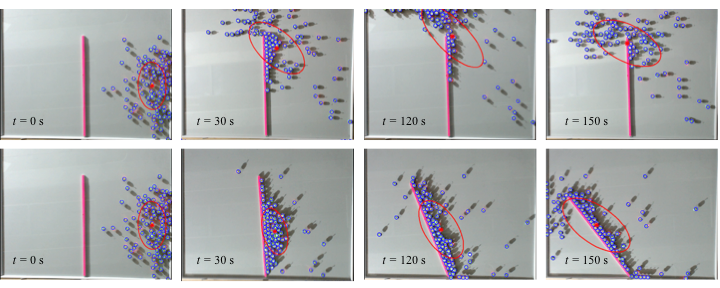
\includegraphics[width=2\columnwidth]{Experiment.png}
\vspace{-1em}
\caption{\label{fig:expBig}{Snapshots showing the effect of pushing a pivoted rectangular object at different distances from the pivot point. 
 97 robots were programmed to move toward the brightest light in the room, and   controlled by choosing which of 8 lights were on at any given instant. The top row of snapshots illustrate the swarm pushing at the end of the object.  In this case,  the swarm flows past the object and the force decreases. The bottom row illustrates that when the swarm pushes at the middle of the object the force provided by the swarm remains constant. In this case the swarm does not flow past the object. See video attachment for recordings of these experiments at\href{https://www.youtube.com/watch?v=ZiKEa5UwukM&feature=youtu.be}{\cite{ShahrokhiTorqueVideo}}.
 }
%\vspace{-2em}
}
\end{figure*}






